% Core stuff: ORM

% LineNumberManager (StoreManager depends for, monitoring, system stop, )
% StoreManager (StoreManager does not need users to function) except AccessErrors & sending emails for timeslot or system stop changes.
% UserManager (SSO, too)

% Self managing thingies:
% OccupancyForecaster
% Mail client

% At one point, frontend middlewares & components, HTTP, Google Maps, QR Code, SSO, Print QR

% ORM (JPA) -> Back-end services (each as a different service Beans (Testable, add mocking to the unittests) -> Routing ) -> Front-end (Logic (Testable, TDD) -> Views (HTML, Snapshot tests))

% Unit tests (TDD), End2End, Browser Emulators conform to standards,

\subsection{Implementation and Integration}
In this section is presented the implementation and integration plan of the entire system, especially the order in which the components are implemented based on their dependencies.\\
The dependencies are shown at three different level of abstraction: entire System, Backend, Services. \\
In the following graphs are shown two types of dependencies: strong dependency and weak dependency.\\
A strong dependency is represented with a continue arrow and represent the fact that the followed component needs the previous one to work.\\
A weak dependency instead is represented with a dashed arrow and indicates that is easier to implement the following component after the previous is completed, but it's not mandatory.\\
\\
\begin{figure}[H]
    \centering
    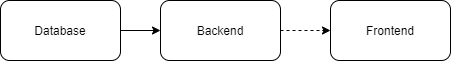
\includegraphics{Images/IntegrationAndTestingPlan/System.png}
    \caption{Entire System}
    \label{fig:System}
\end{figure}

\nameref{fig:System} shows that the Database is the first component to implement, since all the services offered by the backend
need the data stored in the database to work. \\
The frontend can be implemented independently from the backend, but implementing it after the backend is complete is simpler because the interfaces
offered by the backend are completely defined.\\
\\
\begin{figure}[H]
    \centering
    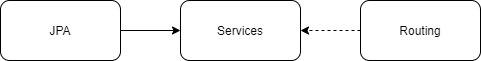
\includegraphics{Images/IntegrationAndTestingPlan/Backend.png}
    \caption{Backend}
    \label{fig:Backend}
\end{figure}
\nameref{fig:Backend} shows how the subcomponents of the Backend component are dependent on each other. \\
In particular we can see that the first component to implement is the ORM component that is needed to map the entities of the database in Objects. This is fundamental because as said before all the services rely on the data in the database and the ORM is
the way used by our system to connect the database to the backend.\\
The REST endpoints define the functionalities of the services that are showed to the user and acts as a bridge from the backend
to the frontend.
This can be implemented independently of the actual services, but it's easier to implement this component before the services because
it can show immediately the functions that need to be implemented.\\
\\
\begin{figure}[H]
    \centering
    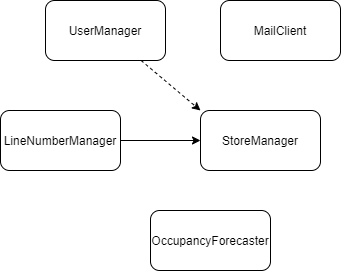
\includegraphics[height=0.4\textwidth]{Images/IntegrationAndTestingPlan/Services.png}
    \caption{Services}
    \label{fig:Services}
\end{figure}
\nameref{fig:Services} defines the order in which the single services are going to be implemented.
The StoreManager depends on the LineNumberManager because it provides the functionalities of monitoring the customers in the store, and the
system stop;
the first one uses the line numbers to count the customers, while the second one needs to invalidate the line numbers
in the time period when the system is stopped.\\
The StoreManager can be implemented independently from the UserManager, but the majority of the functionalities of he StoreManager
are restricted to a specific type of user, so the implementation can be easier if the UserManager is already working properly.
The OccupancyForecaster and the MailClient are completely independent from the other services.\\
\\
\begin{figure}[H]
    \centering
    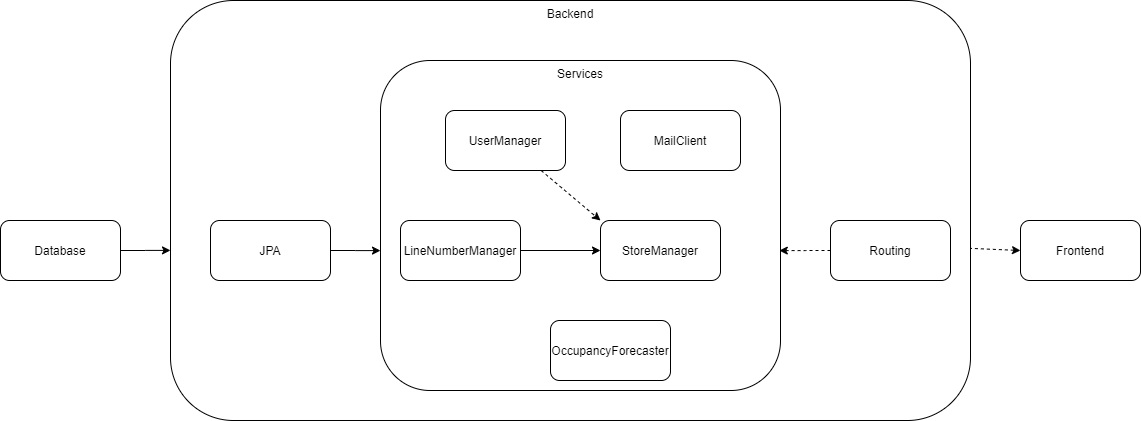
\includegraphics[height=0.4\textwidth]{Images/IntegrationAndTestingPlan/Summary.png}
    \caption{Summary}
    \label{fig:Summary}
\end{figure}
\nameref{fig:Summary} is a summary of the graphs showed before and represent all the dependencies within component in the system.

\subsection{Test plan}
In this section is described how the system will be tested. \\
For which concerns unit testing, the system will be developed using test driven development, so the tests will be written before writing the code.
This is relatively easy for the frontend logic, while requires the implementation of stubs and drivers for the backend modules.
Integration tests are needed only when a new component with a strong dependency, according to the definition of strong dependency
given in the previous section, is added to the system.
Then there will be end to end testing to validate that the components can work together and finally a system test will be performed
using browser emulators conform to standards.
